%%%%%%%%%%%%%%%%%%%%%%%
%%% DOCUMENT SETTINGS
%%%%%%%%%%%%%%%%%%%%%%%
\documentclass[11pt]{exam}
\printanswers % Uncomment to show answers if desired
%%%%%%%%%%%%%%
%%% PACKAGES
%%%%%%%%%%%%%%
\usepackage{amsmath,amsfonts,amssymb,amsthm}  % math fonts and symbols
\usepackage{bbm} % Math blackboard font
\usepackage{enumitem} % Custom list environments
\usepackage{textcomp} % Misc symbols
\usepackage[top=2cm, bottom=2cm, right=1.2cm, left=1.2cm, paper=a4paper, headheight=6cm]{geometry} % Page layout
\usepackage{xcolor}  % Colors
\usepackage{graphicx} % Graphics
%----------------------------------- TikZ
\usepackage{tikz}
\usepackage{pgfplots}
\pgfplotsset{compat=1.17}
\usepgfplotslibrary{fillbetween}
\usetikzlibrary{shapes,arrows,matrix,positioning,calc}
\newcommand{\tikzmark}[1]{\tikz[baseline,remember picture] \coordinate (#1) {};}
%%%%%%%%%%%%%%%%%%%%%%%%%%
%%% COLORS
%%%%%%%%%%%%%%%%%%%%%%%%%%
\definecolor{brickred}{RGB}{200, 50, 50}
\definecolor{skyblue}{RGB}{0, 150, 220}
\definecolor{olivegreen}{RGB}{120, 160, 60}
%%%%%%%%%%%%%%%%%%%%%%%%%%
%%% MACROS
%%%%%%%%%%%%%%%%%%%%%%%%%%
\newcommand{\N}{\mathbb{N}} % natural numbers
\newcommand{\R}{\mathbb{R}} % real numbers
\makeatletter
\renewcommand{\@makefnmark}{\textsuperscript{\arabic{footnote}}}
\renewcommand{\thefootnote}{\arabic{footnote}}
\makeatother
\setcounter{footnote}{0}
\newcommand{\BAR}{%
  \hspace{-\arraycolsep}\strut\vrule\hspace{-\arraycolsep}}
%%%%%%%%%%%%%%%%%%%%%%%%%%%%%%%%%
%%% HEADER AND FOOTER
%%%%%%%%%%%%%%%%%%%%%%%%%%%%%%%%%
% Document information
\newcommand{\degree}{Bachelor in Philosophy, Politics and Economics}
\newcommand{\shortdeg}{PPE}
\newcommand{\exam}{Retake Exam}
\newcommand{\subject}{Mathematics}
\newcommand{\theyear}{2024/25}
\newcommand{\ccauthor}{A. G. Azze}
\newcommand{\thedate}{Jun 9, 2025}
\newcommand{\university}{CUENF Universidad}
% Set header and footer
\pagestyle{headandfoot}
\header{\degree \\ \subject\ - \theyear}{}{\thedate \\ \ccauthor}
\footer{\university}{}{\thepage}
%%%%%%%%%%%%%%%%%%%%%%%%%%
%%% DOCUMENT CONTENT
%%%%%%%%%%%%%%%%%%%%%%%%%%
\begin{document}
%--- Instructions ---%
\begin{center}
    {\Huge \textbf{\exam{}}}
    \begin{flushright}
        \vspace{-0.3cm}
        \textbf{Time Limit:} 120 minutes
    \end{flushright}
    \vspace{-0.2cm}
    \fbox{\parbox{\textwidth}{\centering 
        \begin{enumerate}[leftmargin=0.5cm, label=$\bullet$, rightmargin=0.2cm]
            \item Every non-trivial calculation and claim must be \textbf{justified}.
            % \item Calculators are not necessary and will not be allowed.
            \item Digital devices and internet access are prohibited.
        \end{enumerate}
    }}
\end{center}

%--- Questions ---%

\begin{questions}

%%%%%%%%%%%%%%%%%%%%%%%%%%%%%%%%%%%%%%%%%%%%%%%%%%%%%%%%%%%%%%%%%%%%%
% Question 1: Electric Vehicles Market Analysis
%%%%%%%%%%%%%%%%%%%%%%%%%%%%%%%%%%%%%%%%%%%%%%%%%%%%%%%%%%%%%%%%%%%%%
\question[2.5]
In a market for electric vehicles (EVs), the demand and supply functions are given by
\[
p_D(q) \;=\; 15 - q, 
\qquad
p_S(q) \;=\; 3 + 2q,
\]
where \(q\) is the number of EVs (in thousands of units) and \(p\) is the price (in thousands of dollars) per EV.

\begin{minipage}{0.51\textwidth}
\begin{enumerate}[leftmargin=0.5cm, label=(\alph*), rightmargin=0.2cm]
    \item Find the supply-demand equilibrium \((q^*,p^*)\).
    \item Compute the consumer surplus defined by 
    $$
    CS=\int_{0}^{q^*} p_D(q)\,dq - p^*\,q^*.
    $$
    \item Compute the area denoted by $A$ in Figure 1.
\end{enumerate}
\end{minipage}
\hspace{0.8cm}
\begin{minipage}{0.35\textwidth}
\vspace{-0.1cm}
\begin{center}
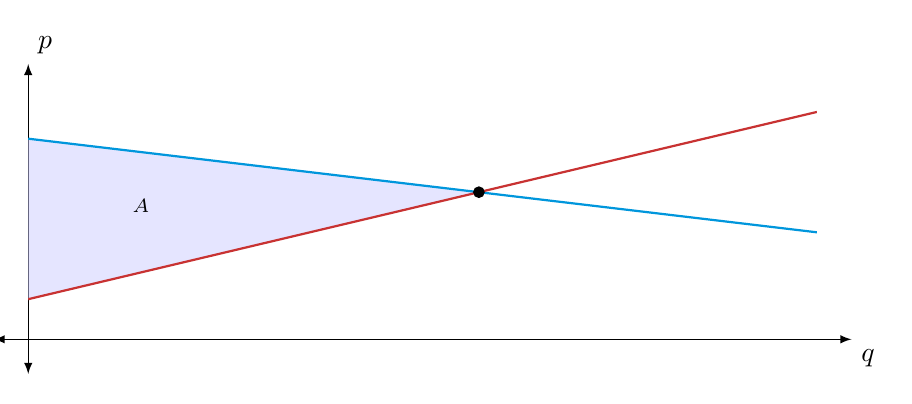
\begin{tikzpicture}[scale=0.95]
    \begin{axis}[
        width=\textwidth,
        height=4.8cm,
        axis lines=middle,
        xmin=0, xmax=7,
        ymin=0, ymax=18,
        xtick={0},
        ytick={0},
        xlabel=$q$,
        ylabel=$p$,
        ticklabel style={font=\scriptsize},
        axis line style={latex-latex, shorten >=-12.5pt, shorten <=-12.5pt},
        xlabel style={at={(ticklabel* cs:1)}, xshift=12.5pt, anchor=north west},
        ylabel style={at={(ticklabel* cs:1)}, yshift=12.5pt, anchor=south west},
    ]
    % Demand curve
    \addplot[thick, skyblue, samples=100, smooth, domain=0:7] {15 - x};
    % Supply curve (only drawn for q between 0 and 4)
    \addplot[thick, brickred, samples=100, smooth, domain=0:7] {3+2*x};
    % Equilibrium point
    \addplot[mark=*] coordinates {(4,11)};
    % Dashed line from equilibrium to axes
    % \addplot[dashed] coordinates {(4,0) (4,11)};
    % \addplot[dashed] coordinates {(0,11) (4,11)};
    % Consumer surplus area
    \path[name path=demand] plot[smooth, domain=0:4] (\x, {15-\x});
    \path[name path=supply] plot[smooth, domain=0:4] (\x, {3+2*\x});
    % \path[name path=price] (axis cs:0,11) -- (axis cs:4,11);
    \addplot[fill=blue!20, opacity=0.5] fill between[of=demand and supply];
    % \node at (axis cs:1.5,13) {\scriptsize $CS$};
    % Label for combined area A (placed arbitrarily)
    \node at (axis cs:1,10) {\scriptsize $A$};
    \end{axis}
\end{tikzpicture}
\vspace{-0.2cm}

{\small Figure 1}
\end{center}
\end{minipage}

\vspace{0.2cm}
To promote greener transportation, the government offers a per-unit subsidy of \(G\) (in dollars) to EV producers, making the new supply-demand equilibrium $q^*(G) = (12 + G)/3$ and $p^*(G) = 11 - G/3$.
\begin{enumerate}[label=(\alph*), leftmargin=0.7cm, start=4]
    \item What values of $G$ will keep the equilibrium price of EVs positive? 
    \item What is the domain of the function $f(G) = q^*(G)/p^*(G)$?
\end{enumerate}

% \begin{minipage}{0.51\textwidth}
Let $M(G) = q^*(G)p^*(G)$ be the total EV market value.
\begin{enumerate}[label=(\alph*), leftmargin=0.7cm, start=6]
    \item What value of $G$ should the government set to maximize the EV market value?
    \item Compute $M'(6)$ and use that value to offer a linear approximation to estimate $M(6.1)$.
\end{enumerate}
% \end{minipage}

\begin{solution}
\begin{enumerate}[label=(\alph*)]
    \item Solving the linear equation $p_D(q)=p_S(q)$ (supply equals demand), we find that the equilibrium quantity is $q^* = 4$, which results in an equilibrium price of $p^* = 11$.
    So, the equilibrium is \((4,11)\).
    
    \item The consumer surplus is given by.
    $$
    CS = \int_{0}^{4} (15 - q)\,dq - 11\times 4 = \left[15q - \frac{q^2}{2}\right]_0^4 - 44= 15\cdot 4 - \frac{4^2}{2} - 44 = 8.
    $$
    
    \item The area \(A\) is the area between the demand and supply curves from $q = 0$ to $q = q^*=4$ is given by
    $$
    A = \int_{0}^{4} \Bigl[(15 - q) - (3 + 2q)\Bigr] \, dq = \int_{0}^{4} (12 - 3q)\,dq = \left[12q - \frac{3q^2}{2}\right]_0^4 = \Bigl[12\cdot 4 - \frac{3\cdot 16}{2}\Bigr] = 48 - 24 = 24.
    $$
    
   \item $p^*(G) = 11-\tfrac{G}{3}>0 \Longleftrightarrow G<33$.
    
    \item $f(G)$ is defined everywhere but for $G$ such that $p^*(G) = 0$. That is, the domain of $f$ is $\R\setminus\{33\}$.
    
    % \item $M(G) = p^*(G)\,q^*(G) = (33-G)(12+G)/9$ is a polynomial in $G$, hence continuous for all real $G$.
    
    \item Since $M'(G)=\frac{21-2G}{9} = 0 \Longleftrightarrow G = 10.5$ and $M''(G) < 0$, then $M(G)$ reaches its maximum at $G = 10.5$.
    
    \item Since $M'(6)=\frac{21-12}{9}=1$ and $M(6) = 54$, the linear approximation at \(G=6\) over a \(0.1\) increase gives
    \[
      M(6.1)\approx M(6)+M'(6)\times 0.1 = 54.1.
    \]
\end{enumerate}
\end{solution}

%%%%%%%%%%%%%%%%%%%%%%%%%%%%%%%%%%%%%%%%%%%%%%%%%%%%%%%%%%%%%%%%%%%%%
% Question 2: Wind Farm Problem
%%%%%%%%%%%%%%%%%%%%%%%%%%%%%%%%%%%%%%%%%%%%%%%%%%%%%%%%%%%%%%%%%%%%%
\question[2.5]
You own a wind farm that produces \(240\) kW of energy each day. Of this:
\[
x = \text{kW injected into the grid},\quad
y = \text{kW stored in a battery},\quad
z = \text{kW consumed on‑site}.
\]
Each kW injected into the grid earns \$5, each kW stored costs \$1 in rental fees, and each kW consumed on‑site “earns” \$0.50 by avoiding purchases.  Your daily net‑revenue goal is \$420.  On stormy days, only half of the grid injection and battery storage and one‑quarter of the on‑site consumption can operate, yet you still need \$195 net revenue.
\begin{enumerate}[leftmargin=0.5cm,label=(\alph*)]
  \item Write the system of equations necessary to find $x$, $y$, and $z$.
  \item Express the system in matrix form, that is, find a matrix $A$ and a vector $\pmb{b}$ such that $A\pmb{w} = \pmb{b}$, for $\pmb{w} = (x, y, z)'$.
  \item Find the values of $x$, $y$, and $z$ that satisfies the system of equations.
  \item What should be the value of $A^{-1}\pmb{b}$? Provide the solution without computing the actual inverse $A^{-1}$.
  \item Imagine now that on stormy days the on‑site consumption operated at half capacity instead of one‑quarter, and that you keep the same net-revenue goal of \$195. Does there exist a solution now?
\end{enumerate}

\begin{solution}
\begin{enumerate}[label=(\alph*)]
  \item The system of equations is
  $$
    \begin{cases}
      x + y + z = 240,\\
      5x - y + 0.5\,z = 420,\\
      2.5\,x - 0.5\,y + 0.125\,z = 195.
    \end{cases}
  $$
  \item In matrix form \(A\mathbf w=\mathbf b\) with
  \[
    A=\begin{pmatrix}
      1   & 1      & 1     \\[3pt]
      5   & -1     & 0.5   \\[3pt]
      2.5 & -0.5   & 0.125
    \end{pmatrix},\quad
    \mathbf w=\begin{pmatrix}x\\y\\z\end{pmatrix},\quad
    \mathbf b=\begin{pmatrix}240\\420\\195\end{pmatrix}.
  \]
  \item Solving (for example by Gaussian elimination) gives
  \[
    x = 80,\quad
    y = 40,\quad
    z = 120.
  \]
  \item Without computing \(A^{-1}\) explicitly, $A^{-1}\,\mathbf b = \begin{pmatrix}80\\40\\120\end{pmatrix}$.
  \item If on stormy days the on‑site consumption ran at half capacity, the third equation would be
  \[
    2.5\,x - 0.5\,y + 0.25\,z = 195,
  \]
  which is exactly half of the second equation \(5x - y + 0.5z = 420\).  Then \(\det A=0\) and the system is inconsistent (because \(2\times195=390\neq420\)), so there is no solution.
\end{enumerate}
\end{solution}

%%%%%%%%%%%%%%%%%%%%%%%%%%%%%%%%%%%%%%%%%%%%%%%%%%%%%%%%%%%%%%%%%%%%%
% Question 3: The WildfIre Problem
%%%%%%%%%%%%%%%%%%%%%%%%%%%%%%%%%%%%%%%%%%%%%%%%%%%%%%%%%%%%%%%%%%%%%
\question[2.5]
A wildfire has broken out at a point in the forest, and your firefighter unit is on the adjacent road when it happens. The closest point on the road to the fire is $\sqrt{27}$ km away.  
Your team can run up to 6 km along the road at 12 km/h, or cut straight through the forest at 6 km/h. As team leader, you decide to run \(x\) km along the road and then head through the forest for the remaining distance. You find that such strategy results in a total time to reach the fire given by the function
\[
T(x) \;=\; \frac{x}{12} \;+\; \frac{\sqrt{(6 - x)^2 + 27}}{6}.
\]

\begin{minipage}{0.57\textwidth}
\begin{enumerate}[leftmargin=0.5cm,label=(\alph*)]
  \item How long would it take to reach the fire if you ran straight through the forest from the start? And if you ran the full 6 km on the road first?
  \item From the graph of $T'(x)$ in Figure 2, how many kilometres \(x\) should you run on the road to minimize the total time? What is the time associated to that optimal value of $x$?
  \item Suppose you cannot enter the forest before the 2 km mark on the road.  What value of \(x\) would you choose now to minimize the total time $T(x)$? And if forest entry is only allowed from the 4 km mark?
\end{enumerate}
\end{minipage}
\hspace{0.8cm}
\begin{minipage}{0.35\textwidth}
\vspace{-0.1cm}
\begin{center}
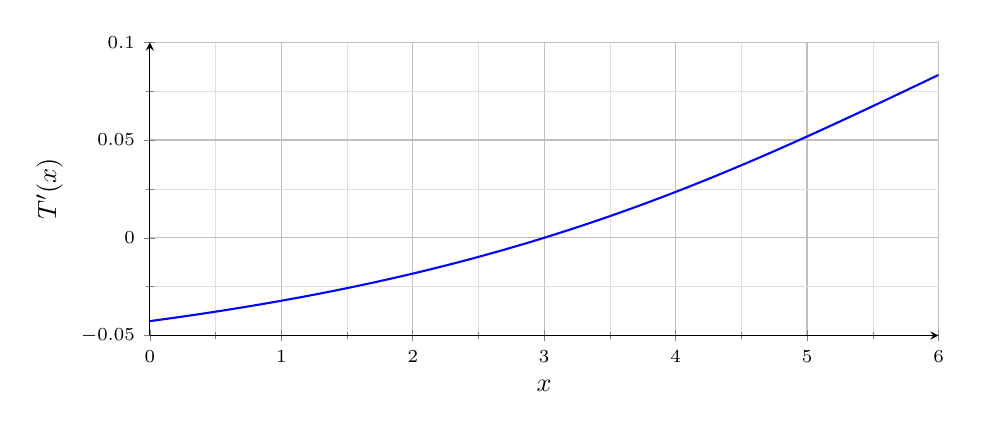
\begin{tikzpicture}[scale=0.95]
  \begin{axis}[
      width=\textwidth,
      height=5.5cm,
      % draw the x‑axis at the bottom (y=-0.05) and the y‑axis at x=0
      axis x line=bottom,
      axis y line=left,
      xmin=0, xmax=6,
      ymin=-0.05, ymax=0.10,
      xtick={0,1,2,3,4,5,6},
      ytick={-0.05,0,0.05,0.1},
      grid=both,
      minor tick num=1,
      major grid style={line width=0.5pt,draw=gray!50},
      minor grid style={line width=0.25pt,draw=gray!25},
      xlabel={$x$},
      ylabel={$T'(x)$},
      ticklabel style={font=\scriptsize},
       ticklabel style={
        font=\scriptsize,
        /pgf/number format/fixed,
        /pgf/number format/precision=3
      },
      scaled ticks=false,
      domain=0:6
    ]
    % Derivative curve
    \addplot[thick, blue, samples=200, smooth] 
      {1/12 - (6 - x)/(6 * sqrt((6 - x)^2 + 27))};
    % Zero line
    % \addplot[dashed, gray] coordinates {(0,0) (6,0)};
    % Mark the root at x=3
    % \addplot[mark=*, mark size=1.5pt] coordinates {(3,0)};
    % \node at (axis cs:3,0.015) [anchor=south] {\scriptsize $x=3$};
  \end{axis}
\end{tikzpicture}
\vspace{-0.5cm}

{\small \hspace{1.3cm} Figure 2}
\end{center}
\end{minipage}

\begin{solution}
\begin{enumerate}[label=(\alph*)]
  \item 
  $
    T(0)
    = \frac{\sqrt{36 + 27}}{6}
    = \frac{\sqrt{63}}{6}
    = \frac{\sqrt7}{2}
    \approx1.323\text{h},
  \quad 
    T(6)
    = \frac{6}{12} + \frac{\sqrt{27}}{6}
    = 0.5 + \frac{\sqrt3}{2}
    \approx1.366\text{h}.
  $
  \item One can note from the graph that $T'(3) = 0$, $T'(x) < 0$ for all $x < 3$, and $T'(x) > 0$ for all $x > 3$, meaning that $x = 3$ is the global minimizer of $T(x)$. The minimum time is then $T(3) = 3/12 + \sqrt{3^2+27}/6 = 1/4 + \sqrt{36/6} = 1.25$.
  \item  If entry $\geq$ 2 km, \(x\in[2,6]\) and the global minimizer \(x=3\) is still allowed, so choose \(x=3\).  
  
  If entry $\geq$ 4 km, \(x\in[4,6]\) and \(3\) is not allowed, so the minimum is at the endpoint \(x=4\).
\end{enumerate}
\end{solution}

%%%%%%%%%%%%%%%%%%%%%%%%%%%%%%%%%%%%%%%%%%%%%%%%%%%%%%%%%%%%%%%%%%%%%
% Question 4: Perpetual Donation Fund Valuation
%%%%%%%%%%%%%%%%%%%%%%%%%%%%%%%%%%%%%%%%%%%%%%%%%%%%%%%%%%%%%%%%%%%%%
\question[2.5]
You own a solar farm with photovoltaic panels whose monthly output slowly declines with age. Let
\(E(t)=10^3e^{-0.05t}\) be the kWh produced in month \(t\). If the market price per kWh in month \(t\) is \(M(t)\) dollars, then your total profit over \(T\) months is
\[
P(T)=\int_{0}^{T}E(t)\,M(t)\,dt.
\]

\begin{enumerate}[leftmargin=0.5cm,label=(\alph*)]
  \item If $M(t)=5e^{0.01t}$,  
    \begin{enumerate}[leftmargin=0.5cm,label=(\roman*)]
      \item Compute the total profit after 10 years, that is, obtain the value of $P(120)$.  
      \item Compute the perpetual profit $\lim_{T\to\infty}P(T) = \int_0^\infty E(t)M(t)\,dt$.
    \end{enumerate}
  \item How long (in months) it will take until you reach a total profit of $P(T) = 5\times10^3$ if $M(t)=e^{-0.05t}$?
  \item For $T=120$ months and $M(t)=5+10^{-3}t$, compute the 10-years total profit $P(120)$. \\
  (Hint: You may use that $f'(t) = (5+10^{-3}t)e^{-0.05t}$ for $f(t) = -(0.02t+100.4)e^{-0.05t}$.)
\end{enumerate}

\begin{solution}
\begin{enumerate}[label=(\alph*)]
  \item If \(M(t)=5e^{0.01t}\), then
  \begin{align*}
      P(T) &= \int_{0}^{T}10^3e^{-0.05t}\times 5e^{0.01t}\,dt
           = 5\times10^3\int_{0}^{T}e^{-0.04t}\,dt \\
           &= \frac{5\times10^3}{0.04}\bigl(1-e^{-0.04T}\bigr)
           = 125\times10^3\bigl(1-e^{-0.04T}\bigr).
  \end{align*}
  \begin{enumerate}[label=(\roman*)]
    \item \(P(120)=125\times10^3\bigl(1-e^{-4.8}\bigr)\approx123.971\times10^3.\)
    \item \(\lim_{T\to\infty}P(T)=125\times10^3.\)
  \end{enumerate}

  \item If \(M(t)=e^{-0.05t}\), then
  \[
    P(T)=\int_{0}^{T}10^3e^{-0.05t}\times e^{-0.05t}\,dt
         =10^3\int_{0}^{T}e^{-0.1t}\,dt
         =\frac{10^3}{0.1}\bigl(1-e^{-0.1T}\bigr)
         =10^4\bigl(1-e^{-0.1T}\bigr).
  \]
  Setting \(P(T)=5\times10^3\) gives \(1-e^{-0.1T}=0.5\), so 
  \[
    e^{-0.1T}=0.5
    \quad\Longrightarrow\quad
    T=-\frac{\ln(0.5)}{0.1}=10\ln2\approx6.93\text{ months}.
  \]

  \item If \(M(t)=5+10^{-3}t\), then
  \[
    P(120)=\int_{0}^{120}10^3e^{-0.05t}\bigl(5+10^{-3}t\bigr)\,dt
           =100.4\times10^3 - 102.8\times10^3\,e^{-6}
           \approx100.145\times10^3
  \]
\end{enumerate}
\end{solution}

\end{questions}	
\end{document}
